\documentclass[11pt]{article}
\usepackage[a4paper,margin=25mm]{geometry}
\usepackage{amsmath,amssymb,bm}
\usepackage{booktabs}
\usepackage{graphicx}
\usepackage{float}
\usepackage{xcolor}
\usepackage{microtype}
\usepackage[hidelinks]{hyperref}

\newcommand{\E}{\mathbb E}
\newcommand{\Dz}{\frac{e^{-z^2/2}}{\sqrt{2\pi}}\,dz}
\newcommand{\mc}{\mu_{\mathrm c}}

\title{The Zero-Effective-Growth Line\\
\large Heterogeneous DMFT for the Relative GLV on a Power-Law Graph}
\author{}
\date{14 July 2026}

\begin{document}
\maketitle

\begin{center}
\fcolorbox{black!35}{blue!4}{\begin{minipage}{0.91\textwidth}
\textbf{Main result.}
The scale equation gives $d\log m/dt=g(t)$ exactly.  On the stationary
heterogeneous-DMFT branch, $g^*=1-a$, so the zero-growth line is obtained by
setting $a=1$ and solving the degree-class closure for $\mc(\sigma)$.  On the
representative $N=4000$ power-law graph, the controlled part of this line ends
at $(\mu,\sigma)\simeq(-0.452,1.023)$.  Its continuation through the unstable
fixed-point regime tracks the measured simulation contour with mean absolute
error $0.029$ in $\mu$ over 23 rows of the production phase grid.
\end{minipage}}
\end{center}

\section{Model and sign convention}

Let
\begin{equation}
  m(t)=\frac1N\sum_{i=1}^N x_i(t),
  \qquad
  S_i(t)=\frac{x_i(t)}{m(t)},
  \qquad
  \frac1N\sum_i S_i(t)=1.
\end{equation}
The relative GLV can be written in absolute variables as
\begin{align}
  \dot x_i &= x_i F_i+\lambda(m-x_i),\\
  F_i &= 1-S_i-\sum_j\beta_{ij}S_j.
  \label{eq:absolute-model}
\end{align}
The mean interaction used by the code is $\mc>0$ for competition.  The plotting
and thesis convention is
\begin{equation}
  \mu=-\mc,
\end{equation}
so stronger competition lies farther to the left in the $(\mu,\sigma)$ plane.

On a graph with adjacency $A_{ij}$, mean degree $C$, and independent standard
Gaussian variables $z_{ij}$, the zero-reciprocity coupling ensemble is
\begin{equation}
  \beta_{ij}
  =A_{ij}\left(\frac{\mc}{C}+\frac{\sigma}{\sqrt C}z_{ij}\right).
  \label{eq:couplings}
\end{equation}

\section{The time dependence of $m(t)$}

This step is essential because $m$ is not a constant.  Since $x_i=mS_i$,
\begin{equation}
  \dot x_i=\dot m\,S_i+m\dot S_i.
  \label{eq:product-rule}
\end{equation}
Averaging Eq.~\eqref{eq:absolute-model}, using $\langle S\rangle=1$, and noting
that the immigration term conserves the mean gives
\begin{align}
  \dot m
  &=\frac1N\sum_i\dot x_i\\
  &=m\frac1N\sum_iS_iF_i
    +\lambda\left(m-\frac1N\sum_i x_i\right)\\
  &=m g(t),
  \qquad
  g(t):=\frac1N\sum_iS_i(t)F_i(t).
  \label{eq:scale-equation}
\end{align}
Substituting Eq.~\eqref{eq:scale-equation} into the product rule yields the
exact relative-size dynamics
\begin{equation}
  \dot S_i=S_i\bigl(F_i-g(t)\bigr)+\lambda(1-S_i).
  \label{eq:share-dynamics}
\end{equation}
The scale itself is therefore
\begin{equation}
  m(t)=m(0)\exp\left[\int_0^t g(s)\,ds\right],
\end{equation}
and the long-time effective growth rate is
\begin{equation}
  \bar g=\lim_{T\to\infty}\frac1T\int_0^Tg(t)\,dt.
  \label{eq:long-run-growth}
\end{equation}

\section{Degree-class heterogeneous DMFT}

Divide vertices into degree classes $p=1,\ldots,n$.  Let $\rho_p$ be the
fraction of vertices in class $p$, let $P_{pr}$ be the probability that a
class-$p$ vertex is linked to a class-$r$ vertex, and define the connectance
$c=C/N$.  It is convenient to introduce
\begin{equation}
  K_{pr}:=\frac{\rho_rP_{pr}}{c}.
  \label{eq:class-kernel}
\end{equation}
For zero reciprocity, the network sum becomes a class-dependent Gaussian field.
The effective process is
\begin{equation}
  \dot S_p
  =S_p\left[1-S_p-\mc B_p(t)+\sigma\eta_p(t)-g(t)\right]
   +\lambda(1-S_p),
  \label{eq:effective-process}
\end{equation}
with
\begin{align}
  B_p(t)&=\sum_rK_{pr}\E[S_r(t)],
  \label{eq:B-dynamic}\\
  \E[\eta_p(t)\eta_p(t')]&=q_p(t,t')
  =\sum_rK_{pr}\E[S_r(t)S_r(t')].
  \label{eq:q-dynamic}
\end{align}
The common scale feedback is fixed self-consistently by
\begin{equation}
  g(t)=\sum_p\rho_p\,
  \E\!\left[S_p(t)\bigl(1-S_p(t)-\mc B_p(t)+\sigma\eta_p(t)\bigr)\right].
  \label{eq:g-dynamic}
\end{equation}
Equations \eqref{eq:effective-process}--\eqref{eq:g-dynamic} are the full
time-dependent heterogeneous theory.  No stationary assumption has yet been
made.

\section{Stationary closure at $\lambda=0$}

In the fixed-point phase, write $g(t)\to g^*$ and
$q_p(t,t')\to q_p^*$.  Define
\begin{equation}
  a:=1-g^*.
  \label{eq:a-definition}
\end{equation}
For a standard normal variable $z$, the stationary abundance is the clipped
Gaussian
\begin{align}
  S_p^*(z)
  &=\left[a-\mc B_p^*+\sigma\sqrt{q_p^*}\,z\right]_+\\
  &=\sigma\sqrt{q_p^*}\,[\Delta_p+z]_+,
  \qquad
  \Delta_p=\frac{a-\mc B_p^*}{\sigma\sqrt{q_p^*}}.
  \label{eq:clipped-law}
\end{align}
Introduce the truncated Gaussian moments
\begin{equation}
  w_n(\Delta)=\int_{-\Delta}^{\infty}\Dz\,(\Delta+z)^n.
\end{equation}
The three moments needed below are
\begin{align}
  w_0(\Delta)&=\Phi(\Delta),\\
  w_1(\Delta)&=\Delta\Phi(\Delta)+\phi(\Delta),\\
  w_2(\Delta)&=(1+\Delta^2)\Phi(\Delta)+\Delta\phi(\Delta).
\end{align}
Therefore
\begin{align}
  \varphi_p&=\Pr(S_p^*>0)=w_0(\Delta_p),\\
  M_{1,p}&=\E[S_p^*]
   =\sigma\sqrt{q_p^*}\,w_1(\Delta_p),\\
  M_{2,p}&=\E[(S_p^*)^2]
   =\sigma^2q_p^*w_2(\Delta_p).
  \label{eq:stationary-moments}
\end{align}
The closure is
\begin{align}
  B_p^*&=\sum_rK_{pr}M_{1,r},
  \label{eq:B-closure}\\
  q_p^*&=\sum_rK_{pr}M_{2,r},
  \label{eq:q-closure}\\
  1&=\sum_p\rho_pM_{1,p},
  \label{eq:normalization}\\
  g^*&=1-a.
  \label{eq:g-fixed}
\end{align}
There are $2n+1$ unknowns, $\{B_p^*,q_p^*\}_{p=1}^n$ and $a$, and exactly
$2n+1$ equations.

\section{Derivation of the $g=0$ line}

The scale equation and Eq.~\eqref{eq:g-fixed} imply
\begin{equation}
  g^*=0
  \quad\Longleftrightarrow\quad
  a=1.
  \label{eq:zero-condition}
\end{equation}
At fixed $\sigma$, impose $a=1$ directly in Eq.~\eqref{eq:clipped-law}:
\begin{equation}
  \Delta_p^{(0)}
  =\frac{1-\mc^{(0)}B_p^{(0)}}
  {\sigma\sqrt{q_p^{(0)}}}.
  \label{eq:delta-zero}
\end{equation}
The unknowns are now
\begin{equation}
  \left\{B_p^{(0)},q_p^{(0)}\right\}_{p=1}^n
  \quad\text{and}\quad \mc^{(0)},
\end{equation}
again $2n+1$ quantities.  They are determined by
\begin{align}
  0&=B_p^{(0)}-\sum_rK_{pr}
  \sigma\sqrt{q_r^{(0)}}w_1(\Delta_r^{(0)}),
  \label{eq:zero-B}\\
  0&=q_p^{(0)}-\sum_rK_{pr}
  \sigma^2q_r^{(0)}w_2(\Delta_r^{(0)}),
  \label{eq:zero-q}\\
  0&=\sum_p\rho_p\sigma\sqrt{q_p^{(0)}}
  w_1(\Delta_p^{(0)})-1.
  \label{eq:zero-normalization}
\end{align}
The line in the thesis sign convention is
\begin{equation}
  \mathcal Z_0
  =\left\{\bigl(-\mc^{(0)}(\sigma),\sigma\bigr):g^*=0\right\}.
  \label{eq:zero-line}
\end{equation}

The implementation uses an equivalent nested procedure.  For each trial
$\mc$, it solves Eqs.~\eqref{eq:B-closure}--\eqref{eq:normalization} for $a$,
computes $g^*=1-a$, and then applies a scalar Brent root search to
\begin{equation}
  g^*(\mc,\sigma)=0.
\end{equation}
In the one-class limit this recovers the homogeneous result
$\mc^{(0)}=g_0(\sigma)$ to numerical precision.

\section{Finite immigration}

For $\lambda>0$, define the Gaussian local field
\begin{equation}
  h_p(z)=a-\mc B_p^*+\sigma\sqrt{q_p^*}\,z.
\end{equation}
The stationary equation is
\begin{equation}
  0=S_p^*(h_p-S_p^*)+\lambda(1-S_p^*),
\end{equation}
or
\begin{equation}
  (S_p^*)^2-(h_p-\lambda)S_p^*-\lambda=0.
\end{equation}
The positive root is
\begin{equation}
  S_p^*(z;\lambda)
  =\frac{h_p(z)-\lambda+
  \sqrt{[h_p(z)-\lambda]^2+4\lambda}}{2}.
  \label{eq:immigration-root}
\end{equation}
The closure retains the same form, but its moments are Gaussian averages of
Eq.~\eqref{eq:immigration-root}.  The zero-growth condition remains $a=1$.

\section{Where the stationary prediction is controlled}

Differentiating the stationary quadratic gives the local susceptibility
\begin{equation}
  \chi_p(z)=\frac{\partial S_p^*}{\partial h_p}
  =\frac{(S_p^*)^2}{(S_p^*)^2+\lambda}.
\end{equation}
Define
\begin{equation}
  R_p(\lambda)=\E_z[\chi_p(z)^2].
\end{equation}
The heterogeneous stability matrix is
\begin{equation}
  \mathcal L_{pr}
  =\sigma^2R_p(\lambda)K_{pr}
  =\frac{\sigma^2}{c}R_p(\lambda)P_{pr}\rho_r.
  \label{eq:stability-matrix}
\end{equation}
The fixed point is stable when
\begin{equation}
  \rho(\mathcal L)<1.
  \label{eq:stability-condition}
\end{equation}
At $\lambda=0$, $R_p=\varphi_p$.  Consequently every point on
$\mathcal Z_0$ must also be tested with Eq.~\eqref{eq:stability-condition}.
The solid segment in Fig.~\ref{fig:zero-growth} is a controlled stationary
prediction.  The dashed segment is the continuation of an unstable fixed
point.

In the fluctuating phase the controlled definition is instead
\begin{equation}
  \bar g=\lim_{T\to\infty}\frac1T\int_0^T
  \sum_p\rho_p\E\!\left[S_p(t)
  \bigl(1-S_p(t)-\mc B_p(t)+\sigma\eta_p(t)\bigr)\right]dt=0,
  \label{eq:dynamic-zero}
\end{equation}
which requires the two-time covariances in Eq.~\eqref{eq:q-dynamic}.  The
stationary continuation may be an accurate approximation, but it is not a
controlled fluctuating-phase derivation.

\section{Numerical result}

The calculation uses a representative graph from the production ensemble:
$N=4000$, target degree $C=100$, power-law exponent $2.5$, graph seed zero,
and 30 equal-population degree bins.  Collapsing the configuration-model
multigraph to a simple graph gives realized mean degree $81.9975$.  The
structural correlations are retained by inverting the soft-configuration
kernel before solving the HDMFT closure.

The zero-growth line meets the fixed-point instability boundary at
\begin{equation}
  (\mu,\sigma)=(-0.451532,\,1.023158).
\end{equation}
All measured phase-grid points shown in Fig.~\ref{fig:zero-growth} lie above
this endpoint.  They must therefore be compared with the dashed continuation,
not with a stable fixed point.

\begin{figure}[H]
  \centering
  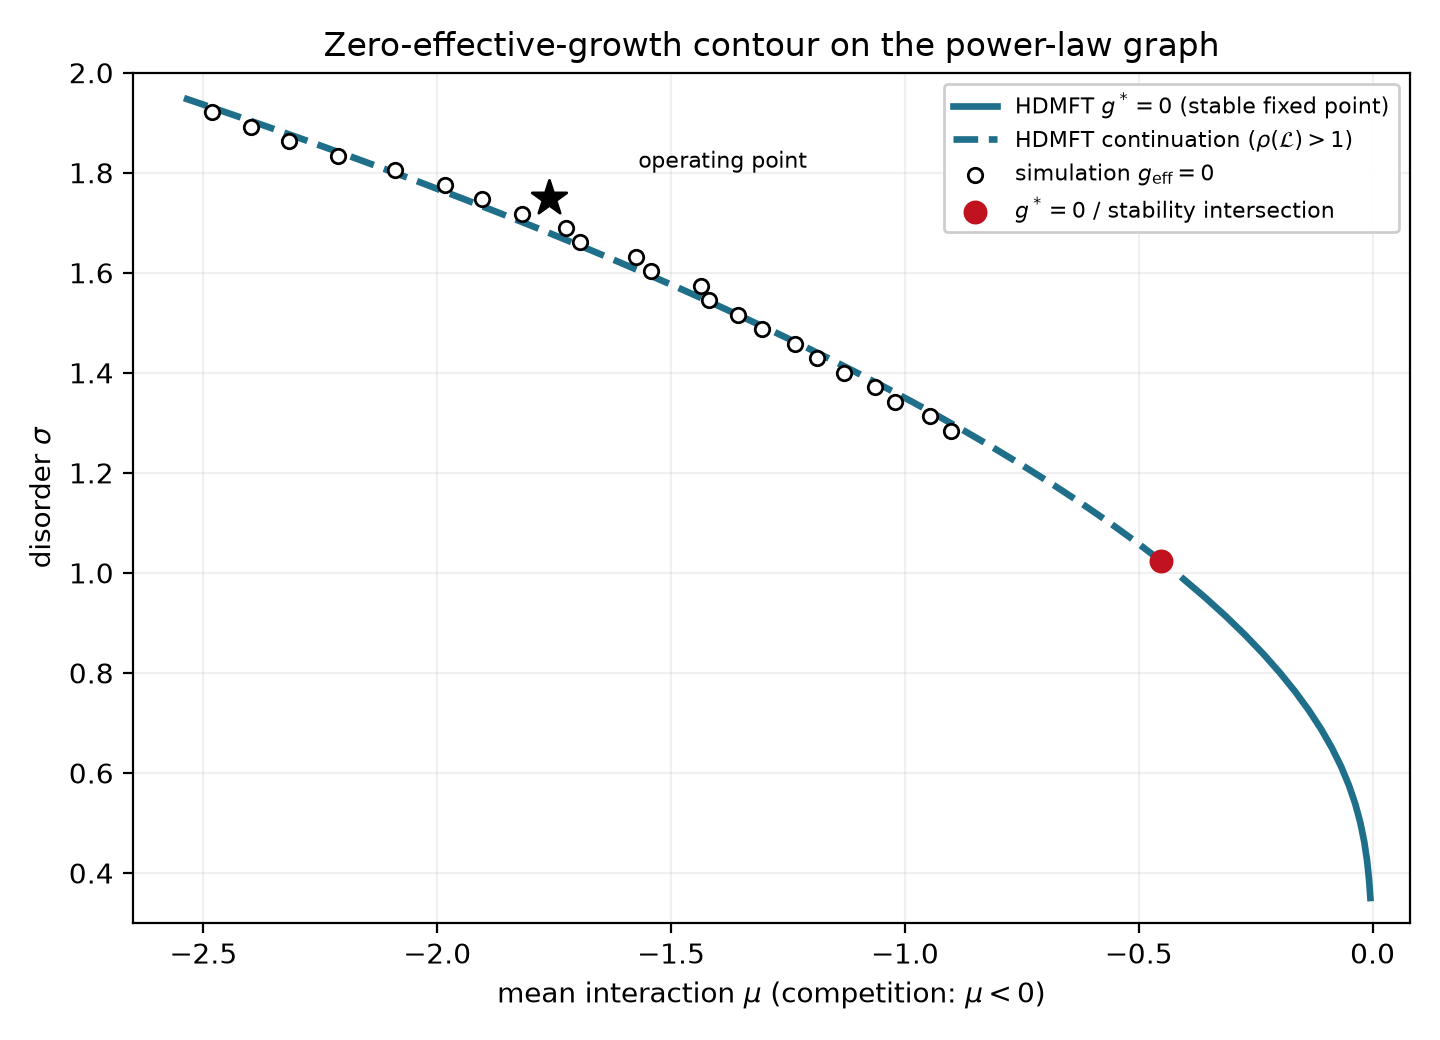
\includegraphics[width=0.96\textwidth]{zero_growth_line.png}
  \caption{The heterogeneous-DMFT zero-growth line and the contour extracted
  from the stored simulation sweep.  Open circles are linear interpolations of
  the median finite-time growth rate through zero at fixed $\sigma$.  The star
  is the operating point $(\mu,\sigma)=(-1.76,1.75)$.}
  \label{fig:zero-growth}
\end{figure}

For the 23 simulation rows containing a sign change, the comparison gives
\begin{align}
  \mathrm{MAE}_{\mu}&=0.02913,\\
  \mathrm{mean}(\mc^{\rm theory}-\mc^{\rm observed})&=0.00262.
\end{align}
Selected values are shown below.  Both columns use the thesis sign convention.
\begin{center}
\begin{tabular}{@{}ccc@{}}
\toprule
$\sigma$ & simulation $\mu$ at $g_{\rm eff}=0$ & HDMFT continuation $\mu$ \\
\midrule
1.2842 & -0.9009 & -0.8734 \\
1.4000 & -1.1297 & -1.1023 \\
1.5737 & -1.4363 & -1.4937 \\
1.7474 & -1.9048 & -1.9434 \\
1.8053 & -2.0910 & -2.1065 \\
1.9211 & -2.4812 & -2.4530 \\
\bottomrule
\end{tabular}
\end{center}

At $\sigma=1.75$, the theoretical continuation gives
$\mu^{(0)}\simeq-1.951$.  The operating point $\mu=-1.76$ lies to the right of
this line and is therefore predicted to have positive effective growth, in
agreement with the simulations.

\clearpage
\section{Conclusion and next theoretical step}

The stationary heterogeneous closure computes a sharply defined $g^*=0$ line
and explains the measured contour surprisingly well.  The essential caveat is
that the relevant production region is already beyond the stability boundary.
Thus the present result has two statuses:
\begin{enumerate}
  \item below $\sigma\simeq1.023$, it is a controlled fixed-point HDMFT result;
  \item above that value, it is an empirically successful unstable-fixed-point
  continuation.
\end{enumerate}
The next step is to solve Eqs.~\eqref{eq:effective-process}--\eqref{eq:q-dynamic}
as a class-resolved two-time stochastic process and impose
Eq.~\eqref{eq:dynamic-zero}.  That calculation will determine whether the close
agreement of the dashed line is asymptotically exact or a finite-time
approximation.

\section*{References}
\begin{enumerate}
  \item A. Aguirre-L\'opez, ``Heterogeneous mean-field analysis of the
  generalized Lotka--Volterra model on a network,'' arXiv:2404.11164 (2024).
  \item S. Patil, A. Altieri, and A. Aguirre-L\'opez, ``Dynamical systems on
  ultra small-world networks,'' arXiv:2605.21364 (2026).
\end{enumerate}

\end{document}
